\indent This experiment was part of a group of four experiments that commissioned the new Hall C Super High Momentum Spectrometer (SHMS) as part of the 12 GeV upgrade at JLab.
A 10.6 GeV electron beam was incident on a 10 cm long liquid deuterium target (LD2). The scattered electron and knocked-out proton were detected in coincidence
by the SHMS and the High Momentum Spectrometer (HMS), respectively. The ``missing'' (undetected) neutron was reconstructed from energy-momentum conservation laws:
$\vec{p_{r}} = \vec{q} - \vec{p_{f}}$ (missing momentum) and $E_{m} = \omega - T_{p} - T_{r}$ (missing energy), where $\vec{p_{f}}$ is the final proton momentum, $(T_{p}, T_{r})$ are the
final proton and neutron kinetic energies, and $E_{m}$ is the binding (missing) energy of the deuteron.
The beam currents delivered by the accelerator ranged between 45-60 $\mu$A and the beam was rastered over a 2x2 mm$^{2}$ area to reduce the effects of localized boiling on the cryogenic targets (hydrogen and deuterium). \\
\indent Both spectrometers at Hall C have similar standard detector packages, each with 1) four scintillator planes\cite{hodo_techreport} used for triggering,
2) a pair of drift chambers\cite{dc_techreport} used for tracking, 3) a calorimeter\cite{Mkrtchyan_2013} used for $e^{-}/\pi^{-}$ discrimination and 4) a gas \u{C}erenkov \cite{Li_Wenliang_mthesis,ngc_techreport} used also for $e^{-}/\pi^{-}$ separation.
Due to the absence of significant background on this experiment and the low coincidence trigger rates
($\sim 1-3$ Hz) at the higher missing momentum settings, the use of additional particle identification (PID) was found to have little to no effect on the final cross section. \\
\indent We measured three central missing momentum settings: $p_{r}=80,580$ and $750$ MeV/c. At each of these settings, the electron arm (SHMS) was fixed and the proton arm (HMS) was rotated from smaller to larger angles corresponding the
the lower and higher missing momentum settings, respectively. At these kinematics, the 3-momentum transfer covered a range of $2.4\lesssim|\vec{q}|\lesssim3.2$ GeV/c which is more than twice the highest neutron recoil momentum ($p_{r}$)
measured on this experiment. As a result, most of the virtual photon momentum is transferred to the proton which scatters at angles relative to $\vec{q}$ in the range $0.4^{o}\lesssim \theta_{pq}\lesssim21.4^{o}$.
At these forward angles and large momentum transferred to the proton, the additional process in which the neutron is struck by the virtual photon is suppressed. \\
\indent Hydrogen elastic $^{1}H(e,e'p)$ data was also taken at kinematics close to the deuteron $p_{r}$=80 MeV setting for cross-checks with the spectrometer acceptance model using the  Hall C Monte Carlo
simulation program, SIMC. Additional $^{1}H(e,e'p)$ data were also taken at three other kinematic settings that covered the SHMS momentum acceptance range for the deuteron and were used for spectrometer optics optimization, 
momentum calibration and the determination of the spectrometer offsets and kinematic uncertainties\cite{cyero_specKinUnc,cyero_SHMSOptics}. \\
\indent Identical event selection criteria were used for the hydrogen and deuteron data. The criteria were determined by making 1) standard cuts on the spectrometer momentum fraction ($\delta$) to select a region in which the reconstruction optics
is well known, 2) a cut to restrict the HMS solid angle acceptance to events that passed directly through the collimator and not by re-scattering from the collimator edges, 3) a missing
energy cut (peak $\sim$ 2.22 MeV for the deuteron) to select true $^{2}H(e,e'p)n$ coincidences, 4) a coincidence time cut to select true coincidence events and not accidentals,  5) a PID cut on the
SHMS calorimeter to select electrons and not other sources of background, mostly pions and 6) a cut on the reconstructed HMS and SHMS reaction vertices to select events that truly
originated from the same reaction vertex at the target. \\
\indent The experimental data yield for both hydrogen and deuteron data was normalized by the total charge and corrected for various inefficiencies. For $^{2}H(e,e'p)n$ the corrections were as follows: tracking efficiencies ($98.9 \%$-HMS, $96.4 \%$-SHMS),
total live time ($92.3 \%$), proton loss due to nuclear interactions in the HMS ($4.7 \%$)\cite{cyero_pAbs} and target boiling factors ($4.2 \%$)\cite{cyero_tgtBoil}. \\
\indent For $^{1}H(e,e'p)$, the corrected data yield was compared to SIMC using J. Arrington's proton form factor parametrization\cite{PhysRevC.69.022201} to check the spectrometer acceptance
model. The ratio of data to simulation yield was determined to be $97.6\pm0.3 \%$ (statistical uncertainty only). For $^{2}H(e,e'p)n$, the low missing momentum data ($p_{r}=80$ MeV/c) were compared to the Hall A data (See Fig. \ref{fig:fig1}).
The good agreement gives us confidence on the measurements made at higher missing momentum settings for which no previous data exist. \\
\indent The systematic uncertainties on the measured cross sections were determined from normalization\footnote{Conservative estimates on the systematic uncertainties of the total live and charge were made.
Determination of systematics on these quantities is a work in progress. (Private communication with D. Mack)} and kinematic uncertainties in the beam energy and spectrometer angle/momentum settings. The individual
contributions from normalization uncertainties were determined to be: tracking efficiencies ($0.40 \%$-HMS, $0.59 \%$-SHMS ), target boiling ($0.39 \%$), total live time ($3.0 \%$) and total charge ($2.0\%$)
for an overall normalization uncertainty added in quadrature of $3.7 \%$. \\
\indent The systematic uncertainties due to our limited knowledge of the beam energy and spectrometer angle/momentum settings were determined point-to-point in ($\theta_{nq}, p_{r}$) bins for each data set independently, and added in quadrature for overlapping $p_{r}$ bins
of different data sets. For $\theta_{nq}=$ 35, 45 and 75 deg (presented on this Letter) the overall kinematic uncertainty varied up to 6.5$\%$ for $p_{r}\leq1.01$ GeV/c.
The overall systematic uncertainty in the cross section was determined by the quadrature sum of the normalization and kinematic uncertainties. This result was then added in quadrature
to the statiscial uncertainty(25-30$\%$ on average) to obtain the final uncertainty in the cross section. \\
\indent The data were radiatively corrected for each bin in ($\theta_{nq}, p_{r}$) by multiplying measured cross sections to the ratio of the SIMC yield without and with radiative effects.
For each bin in ($\theta_{nq}, p_{r}$), the averaged $^{2}H(e,e'p)n$ kinematics has also been calculated and used in the bin centering correction factor defined as:
$f_{bc} \equiv \sigma_{avg.kin} / \bar{\sigma}$, where $\sigma_{avg.kin}$ is the cross section calculated at the averaged kinematics and $\bar{\sigma}$ is the cross
section averaged over the kinematic bin. The calculations were based on the Laget model including FSI\cite{LAGET2005, PhysRevC.21.861}.\\
\indent Both experimental and theoretical reduced cross sections were extracted from the measured (or model) cross 
\onecolumngrid
\begin{center}
\begin{figure}[hb!]
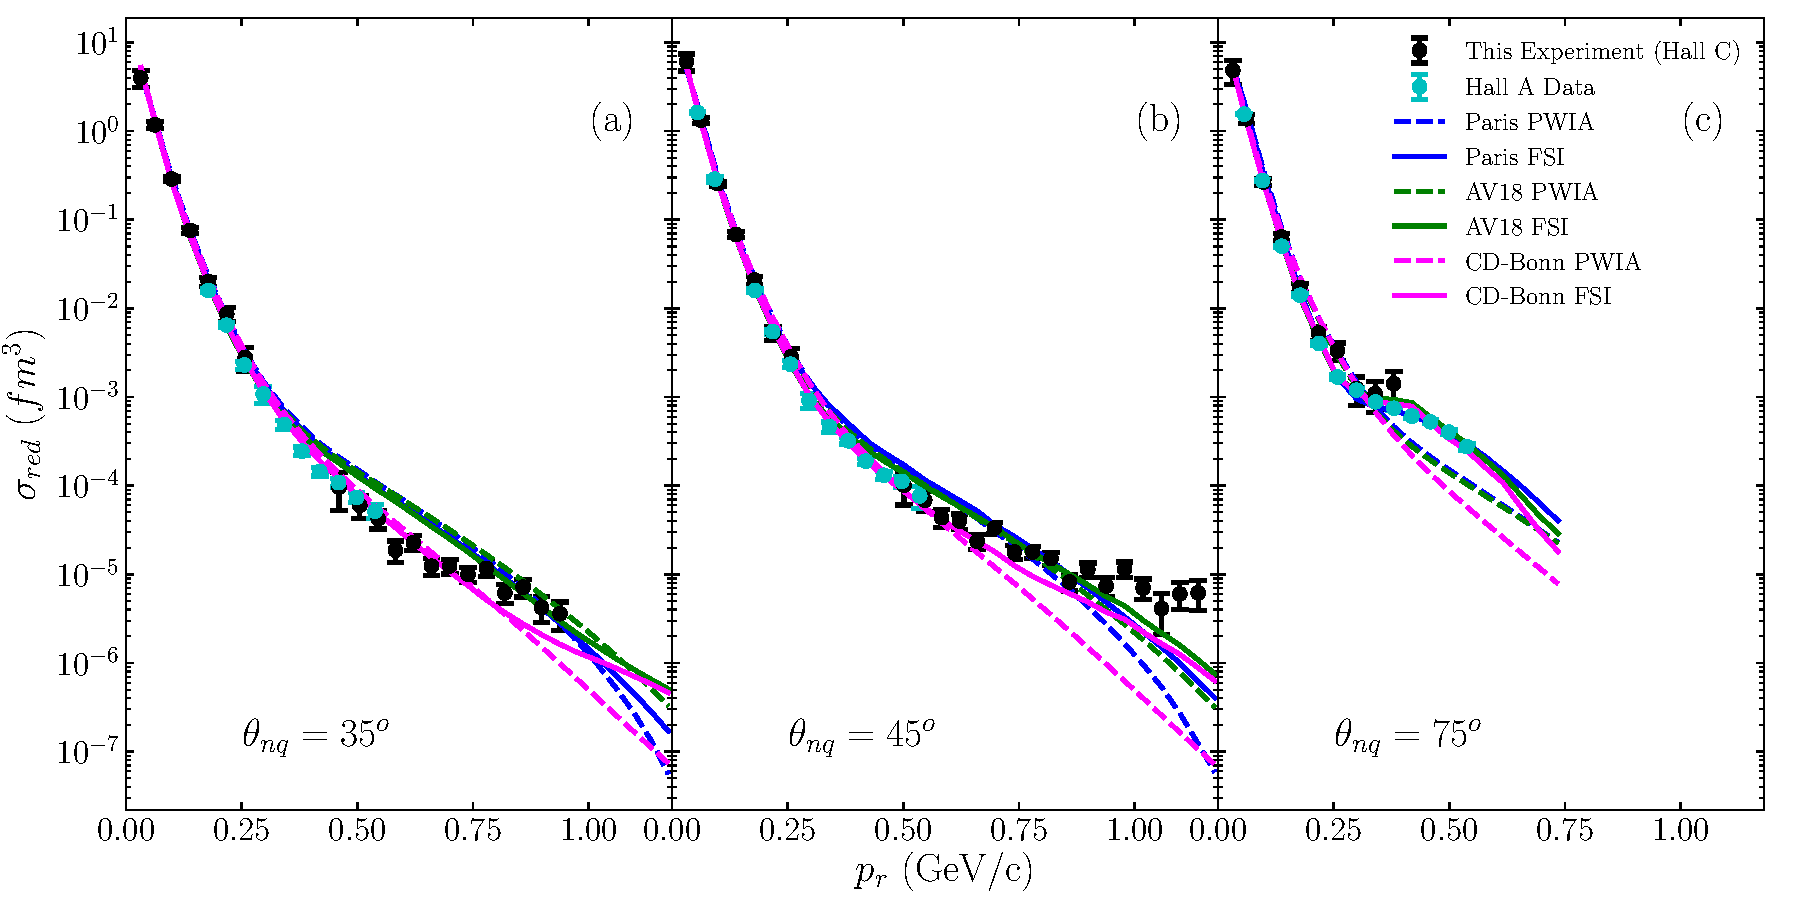
\includegraphics[scale=0.46]{../prl_plots/PRL_plot1.pdf}
\caption{The reduced cross sections $\sigma_{red}(p_{r})$ as a function of neutron recoil momentum $p_{r}$ are shown in (a)-(c) for recoil angles $\theta_{nq}=35^{o}, 45^{o}$ and $75^{o}$, respectively,
with a bin width of $\pm 5^{o}$. The data is compared to the previous Hall A experiment (cyan) results\cite{PhysRevLett.107.262501} as well as the theoretical reduced cross sections using the Paris(blue),
AV18(green) and CD-Bonn(magenta) NN potentials}
\label{fig:fig1}
\end{figure}
\end{center}
\twocolumngrid
\noindent sections for each data set independently and were averaged for overlapping bins in $p_{r}$. The reduced cross sections are defined as follows:
\begin{equation}
\sigma_{red} \equiv \frac{\sigma_{exp(th)}}{Kf_{rec}\sigma_{cc1}}
\label{eq:1}
\end{equation}
where $\sigma_{exp(th)}$ is the 5-fold experimental (or theoretical) differential cross section $\frac{d^{5}\sigma}{d\omega d\Omega_{e} d\Omega_{p}}$, $K$ is a kinematical factor, $f_{rec}$ is the recoil factor that arises from the
integration over missing energy and $\sigma_{cc1}$ is the de Forest\cite{DEFOREST1983} electron-proton offshell cross section calculated using the form factor parametrization of Ref.\cite{PhysRevC.69.022201}.
Within the PWIA, $\sigma_{red}$ corresponds to the proton momentum distribution inside the deuteron. \\
%--------------------------------------EXPLANATION  OF 1ST PLOT (MOMENTUM DISTRIBUTIONS)----------------------------------------
\indent Figure \ref{fig:fig1} shows the extracted experimental and theoretical reduced cross sections as a function of neutron recoil momentum $p_{r}$ for three angular settings at $Q^{2}=4.5\pm0.5$
(GeV/c)$^{2}$. The results from the previous Hall A experiment\cite{PhysRevLett.107.262501} at a $Q^{2}=3.5\pm0.25$ (GeV/c)$^{2}$ are plotted as well (cyan). The data is compared to theoretical reduced
cross sections using the charge-dependent Bonn (CD-Bonn)\cite{PhysRevC.63.024001}, Argonne $v_{18}$ (AV18)\cite{PhysRevC.51.38} and Paris\cite{PhysRevC.21.861} NN-potentials. The theoretical calculations
for the CD-Bonn (magenta) and AV18 (green) potentials were performed by M. Sargsian\cite{PhysRevC.82.014612} and those for the Paris (blue) potential were done by J.M. Laget\cite{LAGET2005}. \\
\indent At recoil angles $\theta_{nq}=75^{o}$ [Fig. \hyperref[fig:fig1]{1(c)}], all models agree and are sensitive to momentum distributions up to $p_{r}\sim$300 MeV/c. Beyond $p_{r}\sim$300 MeV/c, FSIs become
dominant and exhibit a similar behaviour among all models which obscures any possibility of extracting the momentum distributions at these angles. At smaller recoil angles, $\theta_{nq}=35^{o}$ and $45^{o}$ 
[Figs. \hyperref[fig:fig1]{1(a), 1(b)}], the Paris and AV18 calculations show sensitivity to momentum distributions and are within good agreement whereas the CD-Bonn calculation exhibits
a different behaviour beyond $p_{r}\sim$300 MeV/c which indicates a larger sensitivity to the different NN-potentials at higher missing momenta. 


%The data is compared to the results from the previous Hall A experiment\cite{PhysRevLett.107.262501} at a $Q^{2}=3.5\pm0.25$ (GeV/c)$^{2}$.  The overlay of the Hall A data (cyan) in Fig. \ref{fig:fig1}
%provides a continutity to the data from this experiment in the transition from low (80 MeV/c) to high (580, 750) MeV/c missing momentum settings in which there
%was no data. There is also an overall good agreement between the two experiments in the regions in which they overlap in $p_{r}$. \\
%\indent At larger neutron recoil angles of $\theta_{nq}\sim75^{o}$ [Fig. \hyperref[fig:fig1]{1(c)}], the data follows the CD-Bonn PWIA (momentum distributions) up to $p_{r}\sim $100 MeV/c, and at $p_{r}\gtrsim$300 MeV/c, the FSIs become the dominat process and exhibit a
%smaller falloff with $p_{r}$ which obscures any possibility of extracting the momentum distributions. This behaviour of FSI with larger recoil angles was predicted by the GEA\cite{Sargsian_2001,PhysRevC.56.1124} and was verified in previous experiments\cite{PhysRevLett.107.262501,PhysRevLett.98.262502}.
%This experiment kinematics moves away from larger recoil angles and focuses on fowards angles at $\theta_{nq}\sim 40^{o}$ where the momentum distributions become accessible. As a result, our data at larger recoil angles
%is statistically limited. \\
%\indent For recoil angles at $\theta_{nq}=35^{o}$ and $45^{o}$ shown in Figs. \hyperref[fig:fig1]{1(a)} and \hyperref[fig:fig1]{1(b)},  all models predict similar behaviour of the
%momentum distribution for recoil momenta up to $p_{r}\sim$300 MeV/c which the data verifies. At larger $p_{r}$, however, the momentum distributions become increasingly sensitive to the different
%NN potentials, mainly a difference between the CD-Bonn and either the Paris or AV18 is observed. \\
%\indent In Fig. \hyperref[fig:fig1]{1(a)} for example, the data is clearly sensitive to the CD-Bonn momentum distributions between recoil momenta of $300\lesssim p_{r}\lesssim750$ MeV/c before transitioning
%to the Paris/AV18 potentials which is a behaviour that is not well described by any of the models. For recoil angles in Fig. \hyperref[fig:fig1]{1(b)},
%a similar behaviour can be observed, as the data is sensitive to the CD-Bonn momentum distributions but only up to $p_{r}\sim 580$ MeV/c as FSIs start to dominate at lower $p_{r}$ as opposed to Fig. \hyperref[fig:fig1]{1(a)}.
%For $p_{r}>580$ MeV/c, the data again exhibits a behaviour at the high momentum tails which either the CD-Bonn, Paris or AV18 potentials are unable to describe.\\
%---------------------------------------------------------------------------------------------------------------------
%------------The Ratio plot should be shown and explained ONLY after the momentum distribution plot has been shown.--------------
\indent The ratio of the experimental and theoretical reduced cross sections ($\sigma_{red}$) to the deuteron momentum distributions (n$(p_{r})$) is shown in Fig. \ref{fig:fig2}. As a reference we selected the
deuteron momentum distribution calculated using the charge-dependent Bonn (CD-Bonn) potential\cite{PhysRevC.63.024001}.
\begin{figure}[h!]
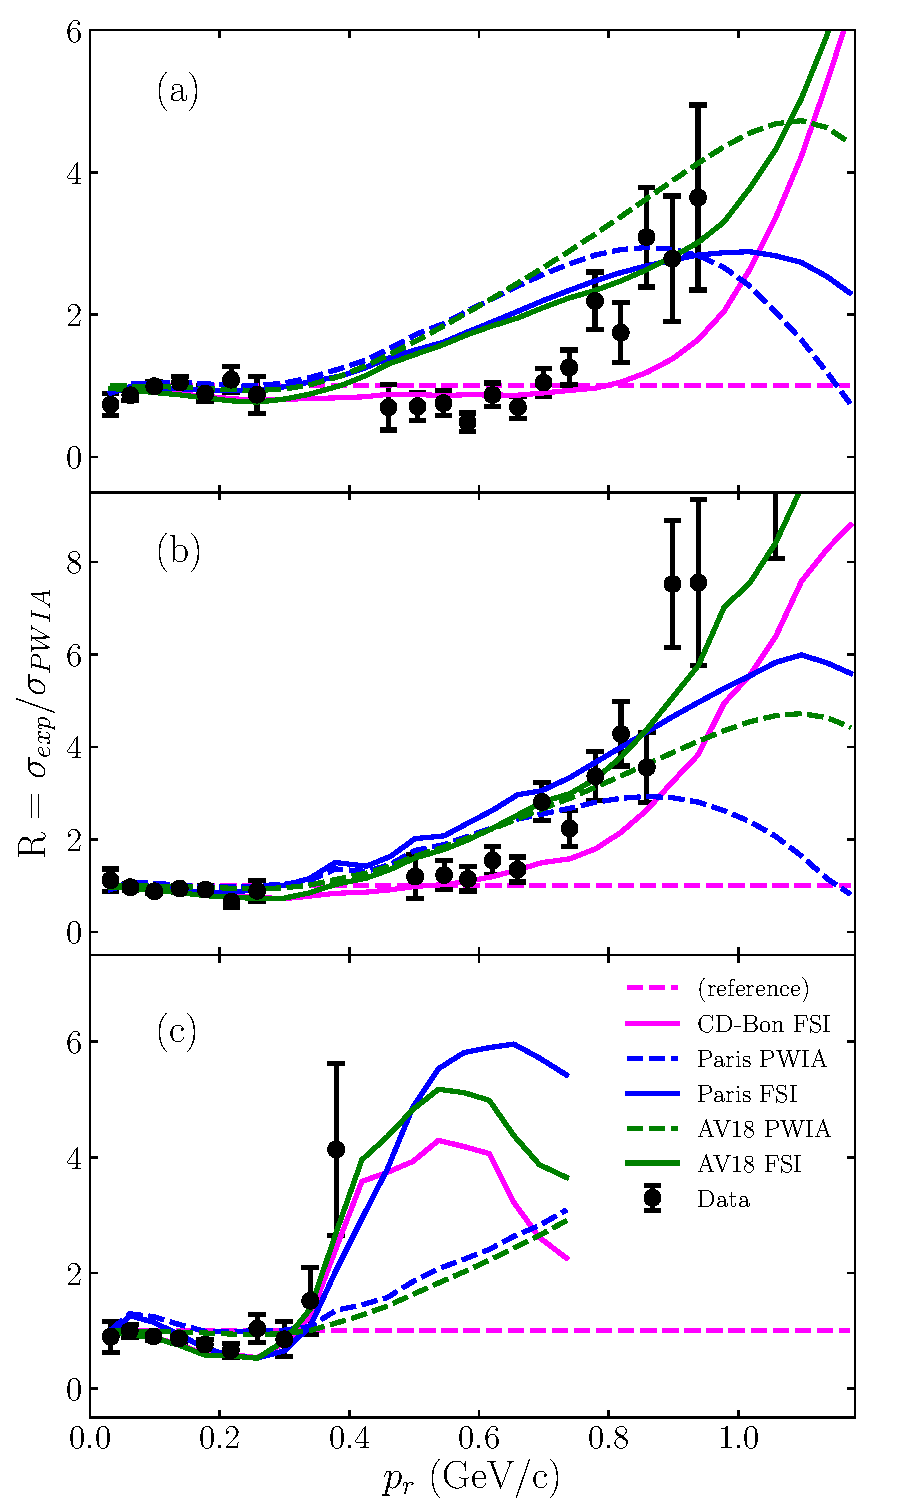
\includegraphics[scale=0.5]{../prl_plots/PRL_plot2.pdf}
\caption{The ratio R($p_{r}$) = $\sigma_{red}$/n$(p_{r})$ is shown in (a)-(c) for $\theta_{nq}=35^{o}, 45^{o}$ and $75^{o}$, respectively, each with a bin width of $\pm 5^{o}$. The dashed reference (magenta) line refers to CD-Bonn momentum distribution (n$(p_{r})$) by which the data and all models are divided. }
\label{fig:fig2}
\end{figure} \\
\indent At $\theta_{nq}=75^{o}$ [Fig. \hyperref[fig:fig2]{2(c)}], there is a clear onset of GEA at $p_{r}\gtrsim300$ MeV/c where FSI become dominant as indicated by the rise of FSI (solid lines) for
all theoretical calculations as compared to the reference. In this region, our experiment is statistically limited as we focused on kinematics at lower recoil angles where FSIs are small. The overlayed
Hall A data, however, shows excellent agreement with the Paris FSI. For $p_{r}<300$ MeV/c, FSIs are small as indicated by the approximate ratio R$\sim$1 for all the theoretical calculations using FSI, which the
data follows. The small dip observed in this region (R$<1$) is indicative of the approximate (not exact) cancellation between the PWIA/FSI interference (screening term) and the modulus-squared of FSI (re-scattering) terms in
the cross section. \\
\indent For $\theta_{nq}=45^{o}$ [Fig. \hyperref[fig:fig2]{2(b)}] at $p_{r}<300$ MeV/c, all theoretical calculations agree with each other and are sensitive to the momentum distribution inside the deuteron which
the data confirms. At $p_{r}\gtrsim300$ MeV/c, the Paris/AV18 calculations start to deviate from the CD-Bonn calculations, with the most substantial deviations observed at $p_{r}\sim 1$ GeV/c.
The CD-Bonn calculations are sensitive to momentum distributions up to $p_{r}\sim$580 MeV/c before FSIs start to dominate (R$>1$).
The data agrees well with the CD-Bonn PWIA calculation but show an earlier rise than predicted by the CD-Bonn FSI, a behaviour which is not described by any of the models. \\
\indent A similar behaviour is observed for $\theta_{nq}=35^{o}$ [Fig. \hyperref[fig:fig2]{2(a)}], where the CD-Bonn calculations are sensitive to momentum distributions up to $p_{r}\sim800$ MeV/c before being
overwhelmed by FSIs, whereas the Paris/AV18 calculations start to deviate from the CD-Bonn at $p_{r}\sim300$ MeV/c. The data shows sensitivity to CD-Bonn momentum distributions up to $p_{r}\sim$750 MeV/c before
exhibiting an earlier rise than predicted by CD-Bonn FSI. \\ 
\indent The $\theta_{nq}=35^{o}$ [Fig. \hyperref[fig:fig2]{2(a)}] appears to be the optimal kinematics to study the high momentum components of the deuteron wavefunction, as the data is sensitive to momentum
distributions up to $p_{r}\sim750$ MeV/c as compared to $p_{r}\sim$580 MeV/c for the $\theta_{nq}=45^{o}$ setting. \\
%-------------------------------------------------------------------------------------------------------------------------------
%----------CONCLUSION----------
\indent This experiment extended the previous Hall A cross section measurements on the $^{2}H(e,e'p)n$ reaction to 
unprecedented large $Q^{2}$ and very high neutron recoil momenta at kinematics that enhanced the high momentum components of the deuteron wavefunction.
The experimental reduced cross sections were extracted and found to be in good agreement with the Hall A data. Furthermore, the CD-Bonn calculations
were found to be sensitive to momentum distributions up to $p_{r}\sim800$ MeV/c for recoil angles $\theta_{nq}=35\pm5^{o}$, which the data agreed
up to $p_{r}\sim750$ MeV/c. At higher missing momentum, however, all models are unable to describe the data, which is currently not well understood.\\
\indent Given that this was a commissioning experiment that ran for only 6 out of the 42 days (14.2$\%$) of beam time and 3 out of the 8 original kinematic settings,
additional beam time would be required to measure the full kinematic coverage (more missing momentum settings) to gain the necessary statistics 
in order to make any definitive arguments about the underlying physics observed. \\
\indent We acknowledge the outstanding support of the staff of the Accelerator and Physics Divisions at Jefferson Lab
as well as the entire Hall C staff, technicians, graduate students and users who took shifts or contributed
to the equipment for the Hall C upgrade making all four commissioning experiments possible. 

%-------------------------------
